\chapter{Force magnétique}
Le magnétisme parle essentiellement de l'influence des charges en mouvement sur d'autres charges en mouvement. Une charge en mouvement crée un champ magnétique et une charge en mouvement placée dans ce champ subit une force appelée : \motcle{force magnétique}.
\section{Force de Lorentz}
La  \motcle{force de Lorentz} est le nom donné à la force magnétique agissant sur une particule chargée se déplaçant au sein d'un champ magnétique. L'expression de cette force est :
\begin{encadre_equation*}{Force de Lorentz}
    \begin{equation}
        \vec{F}=q \cdot \vec{v} \times \vec{B}
    \end{equation} où :
    \begin{itemize}[label=\textbullet]
        \item \(F\) est la force magnétique exercée sur la charge, en \([N]\);
        \item \(q\) est la valeur de la charge, en \([C]\);
        \item \(v\) est la vitesse de la charge, en \([m \cdot s^{-1}]\);
        \item \(B\) est l'intensité du champ magnétique, en \([T]\);
        \item le symbole  \(\times\) désigne un \motcle{produit vectoriel}.
    \end{itemize}
\end{encadre_equation*}
Il est à noter que la valeur de la charge est importante étant donné que le sens de la force de Lorentz sera inverssé pour des particules chargées négativement.

\begin{figure}[h]
    \centering
    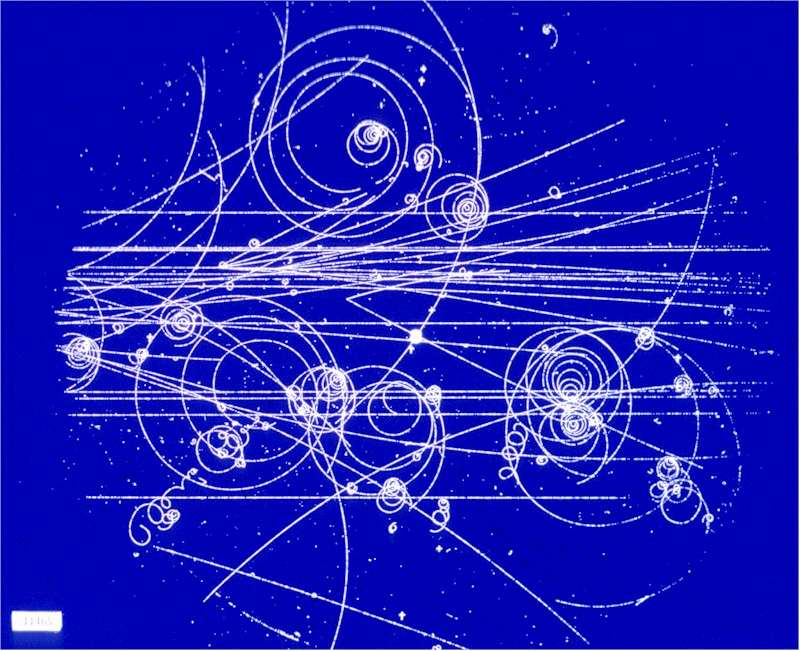
\includegraphics[width=0.8\linewidth]{chambre_bulle.png}
    \caption{Dans une chambre à bulles, des particules chargées circulent dans un champ magnétique, elles subissent une force qui incurve leur trajectoire. le sens de de rotation dépend de la charge de la particule.}
    \label{chambre_bulle}
\end{figure}

\newpage

\section{Force de Laplace}
Lorsqu'un fil conducteur est parcouru par un courant, chaque particule chargée subit une force de Lorentz. l'ensemble du conducteur va donc subir une force qu'on appelle alors \motcle{force de Laplace}. Les caractéristiques de celle-ci sont données par :
\begin{encadre_equation*}{Force de Laplace}
    \begin{equation}
        \vec{F}=I \cdot \vec{l} \times \vec{B}
    \end{equation} où:
    \begin{itemize}[label=\textbullet]
        \item \(F\) est la force de Laplace exercée sur l'élément conducteur, en \([N]\);
        \item \(I\) est l'intensité du courant, en \([A]\);
        \item \(l\) est la longueur de l'élément conducteur, en \([m]\);
        \item \(B\) est l'intensité du champ magnétique, en \([T]\).
    \end{itemize}
\end{encadre_equation*}


\subsection{Produit vectoriel}
Il existe deux opérations de multiplications entre deux vecteurs :
\begin{itemize} [label=\textbullet]
    \item le produit vectoriel
    \item le produit scalaire.
\end{itemize}

Le produit vectoriel de deux vecteurs est un \motcle{vecteur}, il s'applique seulement dans un espace en trois dimensions.

Le produit vectoriel entre  \(\vec{a}\) et \(\vec{b}\) se calcule de la manière suivante :
Si \(\vec{c}=\vec{a} \times \vec{b}\), alors :
\(||\vec{c}||= ||\vec{a}|| \cdot ||\vec{b}|| \cdot sin(\theta)\), où:
\begin{itemize}[label=\textbullet]
    \item \(\theta\) est l'angle qui relie \(\vec{a}\) à \(\vec{b}\) par le plus court chemin,
    \item la direction du vecteur \(\vec{c}\) est toujours perpendiculaire à \(\vec{a}\) et  \(\vec{b}\),
    \item le sens du vecteur \(\vec{c}\) est donné par la règle de la main droite ou la règle du tire-bouchon.
\end{itemize}

\begin{figure}[!ht]
    \centering
    \begin{minipage}[b]{.47\linewidth}
        \centering
        \includegraphics[width=.9\linewidth]{regle_main_droite_II.png}
        \caption{La règle de la main droite appliquée à au cas de la force de Lorentz.}
        \label{regle_main_droite_II}
    \end{minipage}
    \begin{minipage}[b]{.47\linewidth}
        \centering
        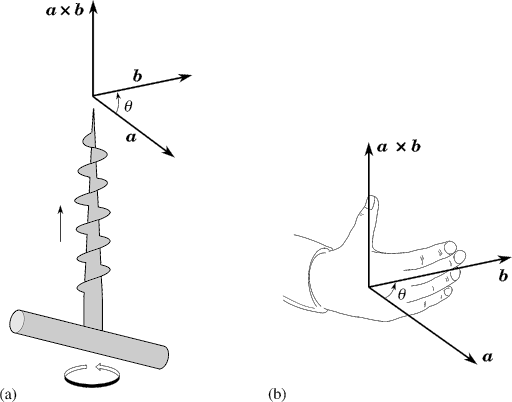
\includegraphics[width=.9\linewidth]{regle_tire_bouchon.png}
        \caption{On fait tourner le premier vecteur vers le second par le côté où c'est le plus court et le sens du vecteur résultat du produit vectoriel est le sens dans lequel le tire-bouchon se déplace.}
        \label{regle_tire_bouchon}
    \end{minipage}
\end{figure}

Pour distinguer un produit vectoriel d'un produit scalaire, le symbole \(\times\) ou \(\wedge\) est utilisé pour le produit vectoriel.

\newpage

\subsection{Produit scalaire}
Le produit scalaire entre deux vecteurs est un \motcle{scalaire}, une valeur non vectorielle.
Le produit scalaire entre \(\vec{a}\) et \(\vec{b}\) se calcule de la manière suivante :
\(c=\vec{a} \cdot \vec{b}= ||\vec{a}|| \cdot ||\vec{b}|| \cdot cos(\theta) \), où :
\begin{itemize}[label=\textbullet]
    \item \(\theta\) est l'angle entre \(\vec{a}\) et \(\vec{b}\).
\end{itemize}
Pour distinguer le produit scalaire du produit vectoriel, le symbole \(\cdot\) est utilisé pour le produit scalaire.
Tu as déjà été confronté plusieurs fois à cette notion, notamment lorsque tu as découvert la notion de travail d'une force, celui-ci correspond au produit scalaire entre le vecteur déplacement et le vecteur force :
\(W=\vec{F} \cdot \vec{\Delta x}\).

\subsection{Vecteur entrant et vecteur sortant}
Lorsqu'on travaille avec des vecteurs orthogonaux dans un espace à trois dimensions, les axes X et Y sont habituellement représentés dans le plan de la feuille sur laquelle on travaille. Il faut cependant pouvoir représenter le sens des vecteurs selon l'axe Z.
\begin{itemize}[label=\textbullet]
    \item Lorsque le sens du vecteur est dirigé vers nous (vecteur sortant), il est symbolisé par \(\bigodot\).
    \item Lorsque le sens du vecteur est dirigé à l'opposé de nous (vecteur entrant), il est symbolisé par \(\bigotimes\).
\end{itemize}
Il faut y voir la représentation d'une flèche qui pointe vers nous et dont on voit la pointe ou qui pointe dans le sens contraire et dont on voit l'empennage.


\begin{figure}[h]
    \centering
    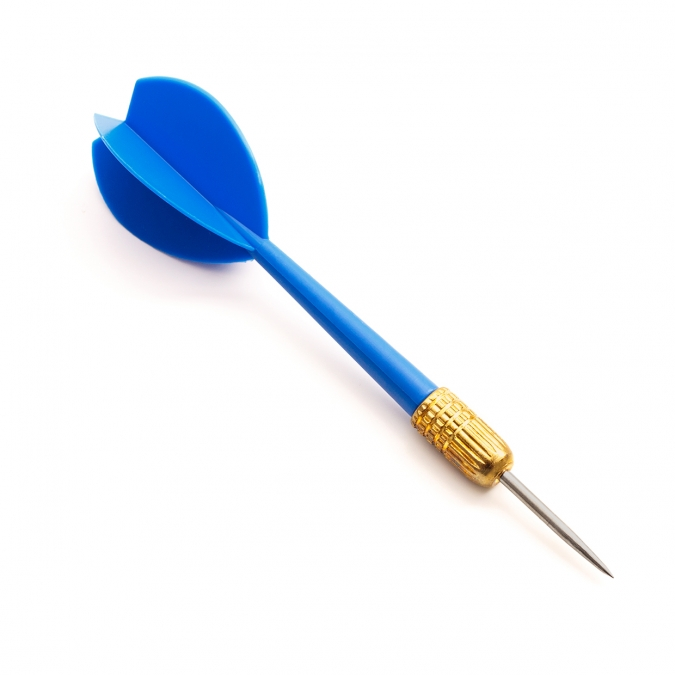
\includegraphics[width=0.4\linewidth]{flechette.png}
    \caption{Une fléchette avec sa point et son empennage.}
    \label{flechette}
\end{figure}

\section{Applications}
\begin{exercise}
    Un barreau en cuivre de \(15cm\) de long et pesant \(50g\) est placé sur un plan incliné formant un angle de \(10^\circ\) vers le haut par rapport à l'horizontale. Ce plan incliné est situé dans un champ magnétique uniforme perpendiculaire au plan et sortant de celui-ci. L'intensité du champ vaut \(0,25[T]\).
    \begin{enumerate}[a)]
        \item Fais un schéma de cette situation.
        \item Dans quel sens le courant doit-il circuler dans le barreau pour qu'il reste en équilibre sur le plan ?
        \item Quelle doit être l'intensité du courant circulant dans le barreau pour qu'il reste en équilibre sur le plan ?
    \end{enumerate}
\end{exercise}

\begin{exercise}
    Un proton se déplace dans le plan XY avec une vitesse de \(50 000km/s\). Dans cette zone, il existe un champ magnétique uniforme de \(0,1 [T]\) dirigé dans le sens positif de l'axe Z.
    \begin{enumerate}[a)]
        \item Quel est le rayon de la trajectoire du proton ? Pour rappel : \(m_{p^+}=1,67 \times 10^{-27} [kg]\) ; \(q_{p^+}=+1,6 \times 10^{-19} [C]\)
        \item dans quel sens tourne-t-il?
    \end{enumerate}
\end{exercise}

\begin{exercise}
    On place une boucle de fil rectangulaire, de dimensions a x l, et porteuse d'un courant I dans un champ magnétique uniforme d'intensité B s'orientant perpendiculairement au plan de la boucle (champ entrant).
    \begin{enumerate}[a)]
        \item Détermine la grandeur et la direction de la force magnétique (force de Laplace) s'exerçant sur chaque côté de la boucle.
        \item Représente ces forces sur un schéma.
        \item Que peux tu prévoir comme comportement pour la boucle ?
        \item Fais le même exercice mais en considérant cette fois que la boucle et les lignes de champ sont parallèles.
    \end{enumerate}
\end{exercise}

\begin{exercise}
    Une boucle de fil rectangulaire de largeur \(L=10[cm]\) parcourue par un courant continu d'intensité \(I=0,245[A]\) est suspendue de manière à ce qu'elle soit partiellement immergée dans un champ magnétique uniforme d'intensité B orienté perpendiculairement au plan de la boucle (champ sortant). La boucle est suspendue à un dynamomètre qui indique une force supplémentaire de \(F=3,48 \times 10^{-2} [N]\) lorsque le courant passe dans le fil. le sens du courant est anti-horloger. Quelle est l'intensité du champ magnétique ?
\end{exercise}


\begin{exercise}
    Un noyeau d'hélium et ses deux électrons pénètrent séparément,en venant de l'est, dans un champ magnétique entrant de \(1,5[T]\) avec une vitesse de \(30000[m/s]\). Réalise un schéma de la trajectoire suivie par ces deux groupes de particules et indique le rayon de courbure pour chacun d'eux.
\end{exercise}

\begin{exercise}
    La balançoire de Laplace.
    Un barreau métallique de \(120[g]\) et de \(30[cm]\) de long est placé dans un champ magnétique uniforme vertical de \(0,1[T]\).
    Ce barreau est suspendu dans le champ grâce à un fil attaché à chacune de ses extrémités de sorte que l'ensemble du dispositif ressemble à une balançoire. Un courant de \(5[A]\) circule dans le barreau. Quel est l'angle formé par les deux fils de suspension?
\end{exercise}

\newpage

\section{Moteurs électrique}
\subsection{Principe de fonctionnement}
Un moteur électrique contient toujours une partie mobile, celle qui tourne, qui est appelée le \motcle{rotor}, la partie fixe est appelée \motcle{stator}.
Si une boucle de fil électrique parcourue par un courant est immergée dans un champ magnétique uniforme parallèle au plan de la boucle alors deux forces de sens opposés s'exercent sur les montants verticaux de la boucle créant ainsi un \motcle{couple de force}.

\begin{figure}[h]
    \centering
    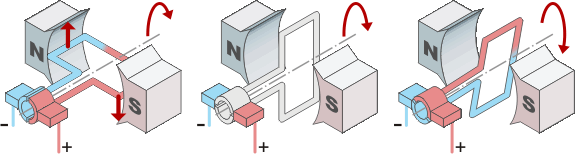
\includegraphics[width=0.7\linewidth]{principe_moteur_dc.png}
    \caption{Principe de fonctionnement d'un moteur à courant continu.}
    \label{principe_moteur_dc}
\end{figure}

\subsubsection*{Premier quart de tour}
Le cadre va alors pivoter sur son axe jusqu'à ce que son plan soit perpendiculaire aux lignes de champs (premier 1/4 de tour). Dans cette configuration, le couple devient nul. Le cadre peut toutefois poursuivre son mouvement grâce à son inertie.

\subsubsection*{Deuxième quart de tour}
Au-delà du premier quart de tour, si le courant circule toujours dans le même sens au sein de la boucle, le couple va s'inverser et la boucle va repartir en sens inverse pour se stabiliser perpendiculairement aux lignes de champs. Il est donc indispensable que le courant s'inverse dans la boucle après le premier quart de tour . C'est le rôle du \motcle{commutateur à balais} : des balais de charbon fixes assurent le contact avec le cadre, lorsque le cadre tourne, le courant s'inverse dans ce dernier et le couple de force est tel qu'il permet de faire tourner le moteur dans le même sens.
Durant le deuxième quart de tour, le couple augmente progressivement.

\begin{figure}[h]
    \centering
    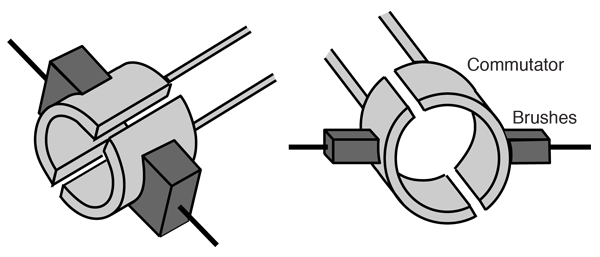
\includegraphics[width=0.4\linewidth]{balais_collecteur.png}
    \caption{Principe de fonctionnement du système balais-collecteur.}
    \label{balais_collecteur}
\end{figure}

\subsubsection*{Troisième quart de tour}
Durant le troisième quart de tour, le sens du courant reste le même que pour le deuxième quart mais la boucle devenant de plus en plus perpendiculaire aux lignes de champs, le couple diminue.


\subsubsection*{Quatrième quart de tour}
Lorsque le dernier quart de tour est entamé, le système du commutateur assure l'inversion du courant dans le cadre et le couple augmente progressivement.

\subsection{Moteurs réels}
Le principe du moteur décrit précédemment comporte plusieurs inconvénients :
\begin{itemize}[label=\textbullet]
    \item la force engendrée par un cadre constitué d'un seul fil est faible ;
    \item le couple de force n'est pas constant ;
    \item le système du commutateur est une source d'usure et les balais de charbon doivent être périodiquement remplacés.
\end{itemize}

Dans un moteur réel, le cadre est donc formé par un fin fil formant de nombreux enroulements et plusieurs cadres sont utilisés afin de maintenir une certaine constance dans le couple.
Actuellement, les moteurs à balais sont de plus en plus souvent remplacés par des moteurs \motcle{brushless} dans lesquels le champ magnétique est généré par des bobines et sa direction est contrôlée électroniquement pour assurer un meilleur couple.

\newpage

\begin{figure}[!ht]
    \centering
    \begin{minipage}[b]{.47\linewidth}
        \centering
        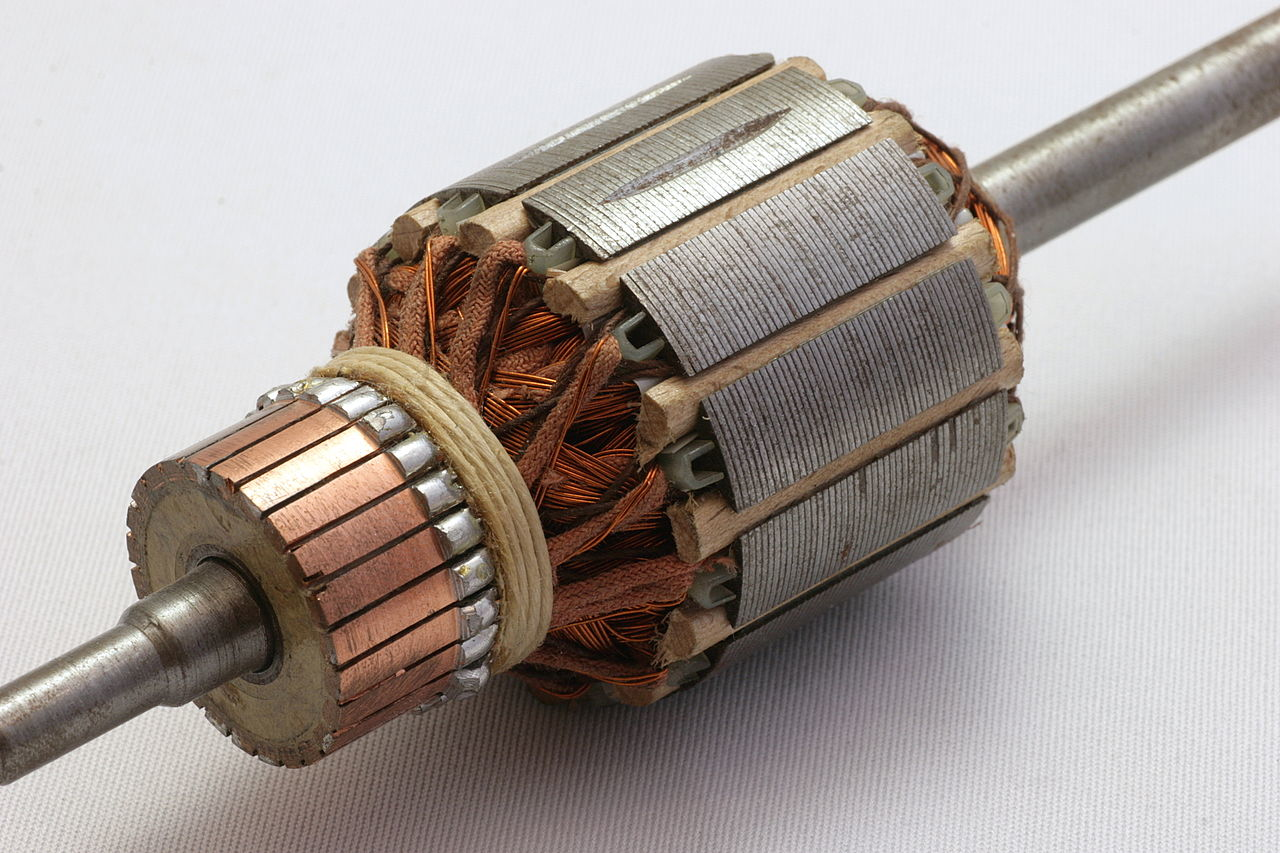
\includegraphics[width=0.9\linewidth]{moteur_universel.png}
        \caption{Un moteur réel.}
        \label{moteur_reel}
    \end{minipage}
    \begin{minipage}[b]{.47\linewidth}
        \centering
        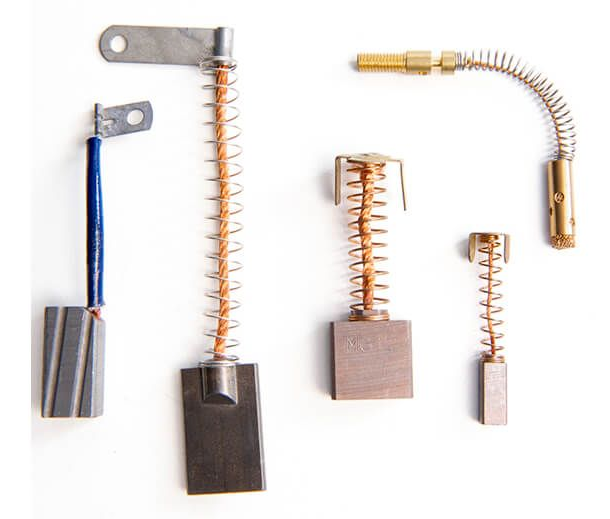
\includegraphics[width=.9\linewidth]{balais_charbon.png}
        \caption{Des balais à charbon de remplacement pour moteur "classique"}
        \label{balais_charbon}
    \end{minipage}
\end{figure}


\begin{figure}[!ht]
    \centering
    \begin{minipage}[b]{.47\linewidth}
        \centering
        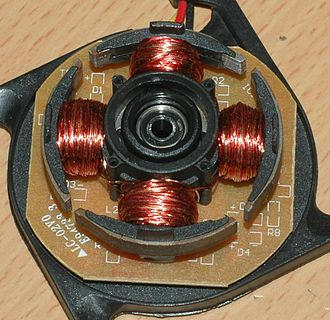
\includegraphics[width=.9\linewidth]{moteur_brushless_I.png}
        \caption{Moteur de ventilateur "brushless".}
        \label{moteur_brushless_I}
    \end{minipage}
    \begin{minipage}[b]{.47\linewidth}
        \centering
        \includegraphics[width=.9\linewidth]{moteur_brushless_II.png}
        \caption{Un moteur brushless de disque dur, les bobines produisant le champ magnétique sont clairement visibles.}
        \label{moteur_brushless_II}
    \end{minipage}
\end{figure}

\newpage

\section{Exercices supplémentaires}
\begin{exercise}
    Détermine la force (par mètre de longueur) qui s'exerce sur un fil droit portant un courant de \(20,5[A]\) et disposé perpendiculairement aux lignes de champ d'un champ magnétique d'une intensité de \(1,8 [T]\). Quelle serait cette force si le fil forme un angle de \(45^\circ\) avec le champ ?
\end{exercise}

\begin{exercise}
    Calcule la force magnétique qui s'exerce sur les \(240[m]\) de fil attachés à deux pylones et portant un courant de \(150[A]\) si le champ magnétique de la Terre vaut \(B=5 \times 10^{-5}[T]\) et forme un angle de \(60^\circ\) avec le fil.
\end{exercise}

\begin{exercise}
    Deux fils rigides parallèles séparés par une distance \(l\) dans un plan horizontal servent de rail à une légère tige métallique de masse \(m\). Un champ magnétique \(B\) uniforme est orienté verticalement vers le haut. À l'instant \(t=0\), on relie les rails à une source de courant continu et le système est parcouru par un courant d'intensité \(I\). Déterminez la vitesse en fonction du temps pour la tige. On suppose que les frottements sont nuls.
\end{exercise}

\begin{exercise}
    Calculez la force qui s'exerce sur un avion ayant acquis une charge de \(150[C]\) lorsqu'il se déplace à une vitesse de \(280[m \cdot s^{-1}]\) perpendiculairement au champ magnétique terrestre d'une intensité de \(B=5 \times 10^{-5}[T]\).
\end{exercise}

\begin{exercise}
    Un projectile de \(7[g]\) se déplace à une vitesse de \(300[m \cdot s^{-1}]\) perpendiculairement au champ magnétique terrestre. Sachant qu'il a une charge nette de \(q=3,5 \times 10^{-9} [C]\), calcule sa déviation de trajectoire sous l'effet du champ magnétique après un parcours de 600[m]. Utilise la loi fondamentale de la dynamique et l'équation horaire du MRUA.
\end{exercise}

